\chapter{\Arrays}
\label{arrays}

\RU{Массив, это просто набор переменных в памяти, 
обязательно лежащих рядом, и обязательно одного типа
\footnote{\ac{AKA} ``гомогенный контейнер''}.}
\EN{An array is just a set of variables in memory 
that lie next to each other and that have the same type
\footnote{\ac{AKA} ``homogeneous container''}.}

% sections
\section{\RU{Простой пример}\EN{Simple example}}

\label{arrays_simple}
\lstinputlisting{patterns/13_arrays/1_simple/simple.c}

\subsection{x86}

\subsubsection{MSVC}

\RU{Компилируем}\EN{Let's compile}:

\lstinputlisting[caption=MSVC 2008]{patterns/13_arrays/1_simple/simple_msvc.asm}

\index{x86!\Instructions!SHL}
\RU{Однако, ничего особенного, просто два цикла, один заполняет цикл, второй печатает его содержимое. 
Команда \TT{shl ecx, 1} используется для умножения \ECX на 2, об этом ниже~(\ref{SHR}).}
\EN{Nothing very special, just two loops: first is filling loop and second is printing loop.
\TT{shl ecx, 1} instruction is used for value multiplication by 2 in the \ECX, more about below~\ref{SHR}.}

\RU{Под массив выделено в стеке $80$ байт, это $20$ элементов по $4$ байта.}
\EN{$80$ bytes are allocated on the stack for array, that is $20$ elements of $4$ bytes.}

\ifdefined\IncludeOlly
\clearpage
\RU{Попробуем этот пример в}\EN{Let's try this example in} \olly.
\index{\olly}

\RU{Видно как заполнился массив}\EN{We see how array gets filled}: 
\RU{каждый элемент это 32-битное слово типа \Tint, с шагом 2}
\EN{each element is 32-bit word of \Tint type, step by 2}:

\begin{figure}[H]
\centering
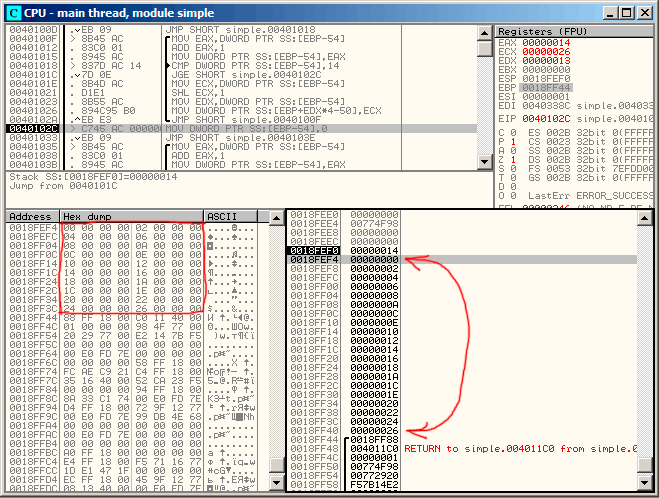
\includegraphics[scale=\FigScale]{patterns/13_arrays/1_simple/olly.png}
\caption{\olly: \RU{после заполнения массива}\EN{after array filling}}
\label{fig:array_simple_olly}
\end{figure}

\RU{А так как этот массив находится в стеке, то мы видим все его 20 элементов внутри стека.}
\EN{Since this array is located in stack, we see all its 20 elements inside of stack.}

\fi

\subsubsection{GCC}

\RU{То, что делает GCC 4.4.1:}\EN{Here is what GCC 4.4.1 does:}

\lstinputlisting[caption=GCC 4.4.1]{patterns/13_arrays/1_simple/simple_gcc.asm}

\RU{Кстати, переменная $a$ в нашем примере имеет тип \IT{int*} (то есть, указатель на \Tint{}) ~--- вы можете попробовать передать в другую функцию указатель на массив, но точнее было бы сказать, что передается указатель на первый элемент массива (а адреса остальных элементов массива можно вычислить очевидным образом).}\EN{By the way, $a$ variable has \IT{int*} type 
(the pointer to \Tint{})~---you can try to pass a pointer to array to another function, but it much correctly to say the pointer to the first array element is passed (addresses of another element's places are calculated in obvious way).}
\RU{Если индексировать этот указатель как \IT{a[idx]}, \IT{idx} просто прибавляется к указателю и возвращается элемент, расположенный там, куда ссылается вычисленный указатель.}\EN{If to index this pointer as \IT{a[idx]}, \IT{idx} just to be added to the pointer and the element placed there (to which calculated pointer is pointing) returned.}

\RU{Вот любопытный пример: строка символов вроде \IT{``string''} это массив из символов, 
и она имеет тип \IT{const char[]}.}\EN{An interesting example: string of characters like 
\IT{``string''} is array of characters and it has \IT{const char[]} type.}
\RU{К этому указателю также можно применять индекc.}
\EN{Index can also be applied to this pointer.}
\RU{И поэтому можно написать даже так:  \TT{``string''[i]} ~--- это совершенно легальное выражение в \CCpp!}
\EN{And that is why it is possible to write like \TT{``string''[i]}~---this is correct \CCpp expression!}

\ifdefined\IncludeARM
\subsection{ARM}

\subsubsection{\NonOptimizingKeilVI (\ARMMode)}

\lstinputlisting{patterns/13_arrays/1_simple/simple_Keil_ARM_O0.asm.\LANG}

\RU{Тип \Tint требует 32 бита для хранения (или 4 байта),}
\EN{\Tint type requires 32 bits for storage (or 4 bytes),}
\RU{так что для хранения 20 переменных типа \Tint, нужно $80$ (\TT{0x50}) байт.}
\EN{so to store 20 \Tint variables $80$ (\TT{0x50}) bytes are needed.}
\RU{Поэтому инструкция}\EN{So that is why the} \TT{\q{SUB SP, SP, \#0x50}} 
\RU{в прологе функции выделяет в локальном стеке под массив именно столько места.}
\EN{instruction in the function's prologie allocates exactly this amount of space in the stack.}

\RU{И в первом и во втором цикле, итератор цикла $i$ будет постоянно находится в регистре \Reg{4}.}
\EN{In both the first and second loops, the loop iterator $i$ is placed in the \Reg{4} register.}

\index{ARM!Optional operators!LSL}
\RU{Число, которое нужно записать в массив, вычисляется так: $i*2$, и это эквивалентно 
сдвигу на 1 бит влево, так что инструкция \TT{\q{MOV R0, R4,LSL\#1}} делает это.}
\EN{The number that is to be written into the array is calculated as $i*2$, which is effectively equivalent 
to shifting it left by one bit, so \TT{\q{MOV R0, R4,LSL\#1}} instruction does this.}

\index{ARM!\Instructions!STR}
\TT{\q{STR R0, [SP,R4,LSL\#2]}} \RU{записывает содержимое \Reg{0} в массив}\EN{writes the contents of \Reg{0} into the array}.
\RU{Указатель на элемент массива вычисляется так: \ac{SP} указывает на начало массива, \Reg{4} это $i$.}
\EN{Here is how a pointer to array element is calculated: \ac{SP} points to the start of the array, \Reg{4} is $i$.}
\RU{Так что сдвигаем $i$ на 2 бита влево, что эквивалентно умножению на $4$ 
(ведь каждый элемент массива занимает 4 байта) и прибавляем это к адресу начала массива.}
\EN{So shifting $i$ left by 2 bits is effectively equivalent to multiplication by $4$
(since each array element has a size of 4 bytes) and then it's added to the address of the start of the array.}

\index{ARM!\Instructions!LDR}
\RU{Во втором цикле используется обратная инструкция \TT{\q{LDR R2, [SP,R4,LSL\#2]}},
она загружает из массива нужное значение, и указатель на него вычисляется точно так же.}
\EN{The second loop has an inverse \TT{\q{LDR R2, [SP,R4,LSL\#2]}}
instruction, it loads the value we need from the array, and the pointer to it is calculated likewise.}

\subsubsection{\OptimizingKeilVI (\ThumbMode)}

\lstinputlisting{patterns/13_arrays/1_simple/simple_Keil_thumb_O3.asm.\LANG}

\RU{Код для thumb очень похожий.}\EN{Thumb code is very similar.}
\index{ARM!\Instructions!LSLS}
\RU{В thumb имеются отдельные инструкции для битовых сдвигов (как \TT{LSLS}), 
вычисляющие и число для записи в массив и адрес каждого элемента массива.}
\EN{Thumb mode has special instructions for bit shifting (like \TT{LSLS}),
which calculates the value to be written into the array and the address of each element in the array as well.}

\RU{Компилятор почему-то выделил в локальном стеке немного больше места, 
однако последние 4 байта не используются.}
\EN{The compiler allocates slightly more space in the local stack, however, the last 4 bytes are not used.}

\subsubsection{\NonOptimizing GCC 4.9.1 (ARM64)}

\lstinputlisting[caption=\NonOptimizing GCC 4.9.1 (ARM64)]{patterns/13_arrays/1_simple/ARM64_GCC491_O0.s.\LANG}

\fi

\section{\RU{Переполнение буфера}\EN{Buffer overflow}}
\label{subsec:bufferoverflow}
\myindex{\BufferOverflow}

\EN{\subsection{Reading outside array bounds}

So, array indexing is just \IT{array\lbrack{}index\rbrack}.
If you study the generated code closely, you'll probably note the missing index bounds checking,
which could check \IT{if it is less than 20}.
What if the index is 20 or greater?
That's the one \CCpp feature it is often blamed for.

Here is a code that successfully compiles and works:

\lstinputlisting{patterns/13_arrays/2_BO/r.c}

Compilation results (MSVC 2008):

\lstinputlisting[caption=\NonOptimizing MSVC 2008]{patterns/13_arrays/2_BO/r_msvc.asm}

The code produced this result:

\begin{figure}[h]
\centering
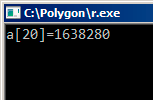
\includegraphics[scale=\NormalScale]{patterns/13_arrays/2_BO/olly_r3.png}
\caption{\olly: console output}
\label{fig:array_BO_olly_r3}
\end{figure}

It is just \IT{something} that was lying in the stack near to the array, 80 bytes away from its first element.

\clearpage
\myindex{\olly}
Let's try to find out where did this value come from, using \olly.

Let's load and find the value located right after the last array element:

\begin{figure}[H]
\centering
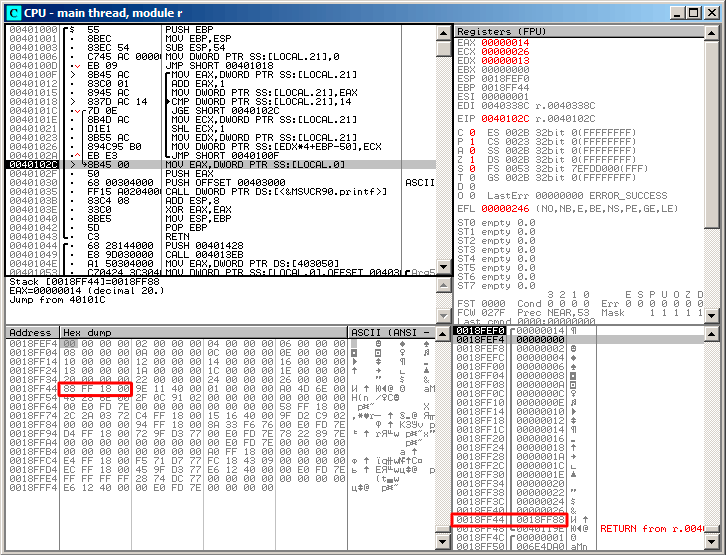
\includegraphics[scale=\FigScale]{patterns/13_arrays/2_BO/olly_r1.png}
\caption{\olly: reading of the 20th element and execution of \printf}
\label{fig:array_BO_olly_r1}
\end{figure}

What is this? 
Judging by the stack layout,
this is the saved value of the EBP register.
\clearpage
Let's trace further and see how it gets restored:

\begin{figure}[H]
\centering
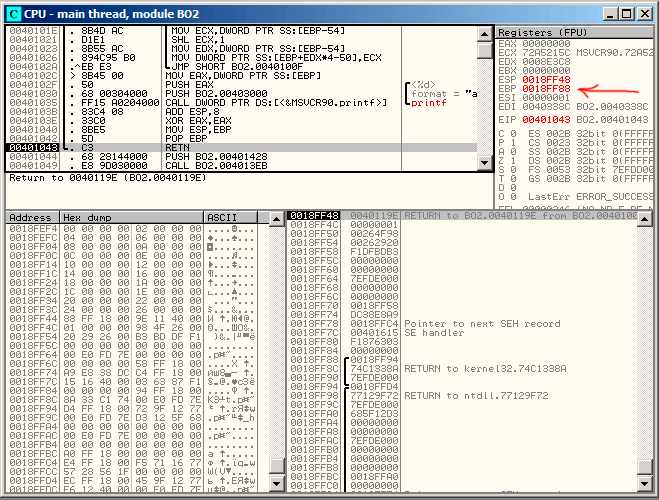
\includegraphics[scale=\FigScale]{patterns/13_arrays/2_BO/olly_r2.png}
\caption{\olly: restoring value of EBP}
\label{fig:array_BO_olly_r2}
\end{figure}

Indeed, how it could be different?
The compiler may generate some additional code to check the index value to be always
in the array's bounds (like in higher-level programming languages\footnote{Java, Python, etc})
but this makes the code slower.

}
\RU{\subsectionold{Чтение за пределами массива}

Итак, индексация массива --- это просто \IT{массив\lbrack{}индекс\rbrack}.  % TODO1 как-то плохо отображаются []
Если вы присмотритесь к коду, в цикле печати значений массива через \printf вы 
не увидите проверок индекса, \IT{меньше ли он двадцати?} 
А что будет если он будет 20 или больше? 
Эта одна из особенностей \CCpp, за которую их, собственно, и ругают.

Вот код, который и компилируется и работает:

\lstinputlisting{patterns/13_arrays/2_BO/r.c}

Вот результат компиляции в (MSVC 2008):

\lstinputlisting[caption=\NonOptimizing MSVC 2008]{patterns/13_arrays/2_BO/r_msvc.asm}

Данный код при запуске выдал вот такой результат:

\begin{figure}[h]
\centering
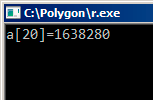
\includegraphics[scale=\NormalScale]{patterns/13_arrays/2_BO/olly_r3.png}
\caption{\olly: вывод в консоль}
\label{fig:array_BO_olly_r3}
\end{figure}

Это просто \IT{что-то}, что волею случая лежало в стеке рядом с массивом, 
через 80 байт от его первого элемента.

\clearpage
\myindex{\olly}
Попробуем узнать в \olly, что это за значение.
Загружаем и находим это значение, находящееся точно после последнего элемента массива:

\begin{figure}[H]
\centering
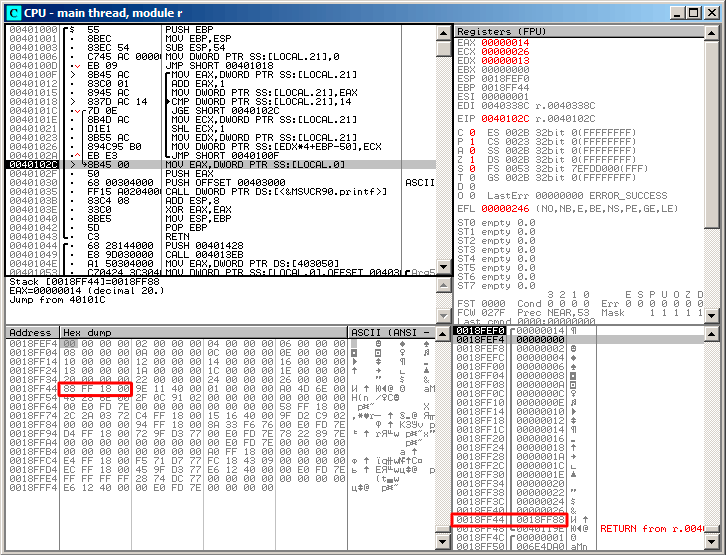
\includegraphics[scale=\FigScale]{patterns/13_arrays/2_BO/olly_r1.png}
\caption{\olly: чтение 20-го элемента и вызов \printf}
\label{fig:array_BO_olly_r1}
\end{figure}

Что это за значение? 
Судя по разметке стека, это сохраненное значение регистра EBP.
\clearpage
Трассируем далее, и видим, как оно восстанавливается:

\begin{figure}[H]
\centering
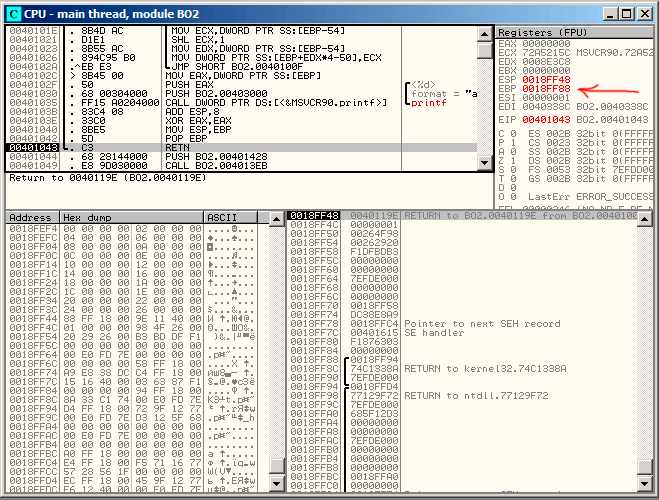
\includegraphics[scale=\FigScale]{patterns/13_arrays/2_BO/olly_r2.png}
\caption{\olly: восстановление EBP}
\label{fig:array_BO_olly_r2}
\end{figure}

Действительно, а как могло бы быть иначе? Компилятор мог бы встроить какой-то код, 
каждый раз проверяющий индекс на соответствие пределам массива, как в языках программирования 
более высокого уровня\footnote{Java, Python, итд.}, что делало бы запускаемый код медленнее.

}
\EN{\subsubsection{Writing beyond array bounds}

OK, we read some values from the stack \IT{illegally}, but what if we could write something to it?

Here is what we have got:

\lstinputlisting{patterns/13_arrays/2_BO/w.c}

\myparagraph{MSVC}

And what we get:

\lstinputlisting[caption=\NonOptimizing MSVC 2008]{patterns/13_arrays/2_BO/w_EN.asm}

The compiled program crashes after running. No wonder. Let's see where exactly does it is crash.

\clearpage
\myindex{\olly}

Let's load it into \olly, and trace until all 30 elements are written:

\begin{figure}[H]
\centering
\myincludegraphics{patterns/13_arrays/2_BO/olly_w1.png}
\caption{\olly: after restoring the value of EBP}
\label{fig:array_BO_olly_w1}
\end{figure}

\clearpage
Trace until the function end:

\begin{figure}[H]
\centering
\myincludegraphics{patterns/13_arrays/2_BO/olly_w2.png}
\caption{\olly: 
EIP was restored, but \olly can't disassemble at 0x15}
\label{fig:array_BO_olly_w2}
\end{figure}

Now please keep your eyes on the registers.

\EIP is 0x15 now. It is not a legal address for code---at least for win32 code!
We got there somehow against our will.
It is also interesting that the \EBP register contain 0x14,
\ECX and \EDX contain 0x1D.

Let's study stack layout a bit more.

After the control flow was passed to \TT{\main}, the value in the \EBP register was saved on the stack.
Then, 84 bytes were allocated for the array and the $i$ variable.
That's \TT{(20+1)*sizeof(int)}.
\ESP now points to the \TT{\_i} variable in the local stack and after the execution of 
the next \TT{PUSH something}, \IT{something} is appearing next to \TT{\_i}.

That's the stack layout while the control is in \main:

\begin{center}
\begin{tabular}{ | l | l | }
\hline
  \TT{ESP}    & 4 bytes allocated for $i$ variable \\
\hline
  \TT{ESP+4}  & 80 bytes allocated for \TT{a[20]} array \\
\hline
  \TT{ESP+84} & saved \EBP value \\
\hline
  \TT{ESP+88} & return address \\
\hline
\end{tabular}
\end{center}

\TT{a[19]=something} statement writes the last \Tint in the bounds of the array (in bounds so far!).

\TT{a[20]=something} statement writes \IT{something} to the place where the value of \EBP is saved.

Please take a look at the register state at the moment of the crash. In our case,
20 was written in the 20th element. 
At the function end, the function epilogue restores the original \EBP value.
(20 in decimal is \TT{0x14} in hexadecimal).
Then \RET gets executed, which is effectively equivalent to \TT{POP EIP} instruction.

The \RET instruction takes the return address from the stack (that is the address in \ac{CRT}),
which was called \main),
and 21 iss stored there (\TT{0x15} in hexadecimal).
The CPU traps at address \TT{0x15},
but there is no executable code there, so exception gets raised.

\myindex{\BufferOverflow}

Welcome! It is called a \IT{buffer overflow}\footnote{\href{http://go.yurichev.com/17132}{wikipedia}}.

Replace the \Tint array with a string (\Tchar array), create a long string deliberately
and pass it to the program, to the function, which doesn't check the length of the string and copies it in a short buffer,
and you'll able to point the program to an address to which it must jump.
It's not that simple in reality, but that is how it emerged.
Classic article about it: \AlephOne.

\myparagraph{GCC}

Let's try the same code in GCC 4.4.1. We get:

\lstinputlisting{patterns/13_arrays/2_BO/w_gcc.asm}

Running this in Linux will produce: \TT{Segmentation fault}.

\myindex{GDB}

If we run this in the GDB debugger, we get this:

\begin{lstlisting}
(gdb) r
Starting program: /home/dennis/RE/1 

Program received signal SIGSEGV, Segmentation fault.
0x00000016 in ?? ()
(gdb) info registers
eax            0x0	0
ecx            0xd2f96388	-755407992
edx            0x1d	29
ebx            0x26eff4	2551796
esp            0xbffff4b0	0xbffff4b0
ebp            0x15	0x15
esi            0x0	0
edi            0x0	0
eip            0x16	0x16
eflags         0x10202	[ IF RF ]
cs             0x73	115
ss             0x7b	123
ds             0x7b	123
es             0x7b	123
fs             0x0	0
gs             0x33	51
(gdb) 
\end{lstlisting}

The register values are slightly different than in win32 example, 
since the stack layout is slightly different too.

}
\RU{\subsectionold{Запись за пределы массива}

Итак, мы прочитали какое-то число из стека явно \IT{нелегально}, а что если мы запишем?

Вот что мы пишем:

\lstinputlisting{patterns/13_arrays/2_BO/w.c}

\subsubsectionold{MSVC}

И вот что имеем на ассемблере:

\lstinputlisting[caption=\NonOptimizing MSVC 2008]{patterns/13_arrays/2_BO/w_RU.asm}

Запускаете скомпилированную программу, и она падает. Немудрено. Но давайте теперь узнаем, где именно.

\clearpage
\myindex{\olly}

Загружаем в \olly, трассируем пока запишутся все 30 элементов:

\begin{figure}[H]
\centering
\myincludegraphics{patterns/13_arrays/2_BO/olly_w1.png}
\caption{\olly: после восстановления EBP}
\label{fig:array_BO_olly_w1}
\end{figure}

\clearpage
Доходим до конца функции:

\begin{figure}[H]
\centering
\myincludegraphics{patterns/13_arrays/2_BO/olly_w2.png}
\caption{\olly: EIP восстановлен, но \olly не может дизассемблировать по адресу 0x15}
\label{fig:array_BO_olly_w2}
\end{figure}

Итак, следите внимательно за регистрами.

\EIP теперь 0x15. Это явно нелегальный адрес для кода~--- по крайней мере, win32-кода! 
Мы там как-то очутились, причем, сами того не хотели. Интересен также тот факт, что в \EBP хранится 0x14, 
а в \ECX и \EDX хранится 0x1D.

Ещё немного изучим разметку стека.

После того как управление передалось в \main, в стек было сохранено значение \EBP. 
Затем для массива и переменной $i$ было выделено 84 байта. Это \TT{(20+1)*sizeof(int)}. 
\ESP сейчас указывает на переменную \TT{\_i} в локальном стеке и при исполнении следующего \INS{PUSH что-либо}, 
\IT{что-либо} появится рядом с \TT{\_i}.

Вот так выглядит разметка стека пока управление находится внутри \main:

\begin{center}
\begin{tabular}{ | l | l | }
\hline
  \TT{ESP}    & 4 байта выделенных для переменной $i$ \\
\hline
  \TT{ESP+4}  & 80 байт выделенных для массива \TT{a[20]} \\
\hline
  \TT{ESP+84} & сохраненное значение \EBP \\
\hline
  \TT{ESP+88} & адрес возврата \\
\hline
\end{tabular}
\end{center}

Выражение \TT{a[19]=что\_нибудь} записывает последний \Tint в пределах массива (пока что в пределах!).

Выражение \TT{a[20]=что\_нибудь} записывает \IT{что\_нибудь} на место где сохранено значение \EBP.

Обратите внимание на состояние регистров на момент падения процесса. В нашем случае 
в 20-й элемент записалось значение 20. 
И вот всё дело в том, что заканчиваясь, эпилог функции восстанавливал значение \EBP 
(20 в десятичной системе это как раз \TT{0x14} в шестнадцатеричной). 
Далее выполнилась инструкция \RET, которая на самом деле эквивалентна \TT{POP EIP}.

Инструкция \RET вытащила из стека адрес возврата (это адрес где-то внутри \ac{CRT}), которая вызвала \main),
а там было записано 21 в десятичной системе, то есть 0x15 в шестнадцатеричной. 
И вот процессор оказался по адресу 0x15, но исполняемого кода там нет, так что случилось исключение.

\myindex{\BufferOverflow}
Добро пожаловать! Это называется \IT{buffer overflow}\footnote{\href{http://go.yurichev.com/17132}{wikipedia}}.

Замените массив \Tint на строку (массив \Tchar), нарочно создайте слишком длинную строку, 
передайте её в ту программу, 
в ту функцию, которая не проверяя длину строки скопирует её в слишком короткий буфер, 
и вы сможете указать программе, по какому именно адресу перейти. 
Не всё так просто в реальности, конечно, но началось всё с этого.
Классическая статья об этом: \AlephOne.

\subsubsectionold{GCC}

Попробуем то же самое в GCC 4.4.1. У нас выходит такое:

\lstinputlisting{patterns/13_arrays/2_BO/w_gcc.asm}

Запуск этого в Linux выдаст: \TT{Segmentation fault}.

\myindex{GDB}
Если запустить полученное в отладчике GDB, получим:

\begin{lstlisting}
(gdb) r
Starting program: /home/dennis/RE/1 

Program received signal SIGSEGV, Segmentation fault.
0x00000016 in ?? ()
(gdb) info registers
eax            0x0	0
ecx            0xd2f96388	-755407992
edx            0x1d	29
ebx            0x26eff4	2551796
esp            0xbffff4b0	0xbffff4b0
ebp            0x15	0x15
esi            0x0	0
edi            0x0	0
eip            0x16	0x16
eflags         0x10202	[ IF RF ]
cs             0x73	115
ss             0x7b	123
ds             0x7b	123
es             0x7b	123
fs             0x0	0
gs             0x33	51
(gdb) 
\end{lstlisting}

Значения регистров немного другие, чем в примере win32, потому что разметка стека чуть другая.

}


\section{\RU{Защита от переполнения буфера}\EN{Buffer overflow protection methods}}
\label{subsec:BO_protection}

\RU{В наше время пытаются бороться с этой напастью, не взирая на халатность программистов на \CCpp. 
В MSVC есть опции вроде}
\EN{There are several methods to protect against it, regardless of \CCpp programmers' negligence.
MSVC has options like}\footnote{
Wikipedia: \RU{описания защит, которые компилятор может вставлять в код}
\EN{compiler-side buffer overflow protection methods}:\\
\url{http://en.wikipedia.org/wiki/Buffer_overflow_protection}}:

\begin{lstlisting}
 /RTCs Stack Frame runtime checking
 /GZ Enable stack checks (/RTCs)
\end{lstlisting}

\index{x86!\Instructions!RET}
\index{Function prologue}
\index{Security cookie}
\RU{Один из методов, это в прологе функции вставлять в область локальных переменных 
некоторое случайное значение 
и в эпилоге функции, перед выходом, это число проверять. 
И если проверка не прошла, то не выполнять инструкцию \RET а остановиться (или зависнуть). 
Процесс зависнет, но это лучше, чем удаленная атака на ваш хост.}
\EN{One of the methods is to write random value among local variables to stack at function prologue 
and to check it in function epilogue before function exiting.
And if value is not the same, do not execute last instruction \RET, but halt (or hang).
Process will hang, but that is much better then remote attack to your host.}
    
\newcommand{\CANARYURL}
{
    \RU
    {
        \url{http://miningwiki.ru/wiki/\%D0\%9A\%D0\%B0\%D0\%BD\%D0\%B0\%D1\%80\%D0\%B5\%D0\%B9\%D0\%BA\%D0\%B0_\%D0\%B2_\%D1\%88\%D0\%B0\%D1\%85\%D1\%82\%D0\%B5}
    }
    \EN{
        \url{http://en.wikipedia.org/wiki/Domestic\_Canary\#Miner.27s\_canary}
    }
}

\index{Canary}
\RU{Это случайное значение иногда называют ``канарейкой''
\footnote{``canary'' в англоязычной литературе}, 
по аналогии с шахтной канарейкой\footnote{\CANARYURL},
их использовали шахтеры в свое время, чтобы определять, есть ли в шахте опасный газ.
}
\EN{This random value is called ``canary'' sometimes, it is related to miner's canary\footnote{\CANARYURL},
they were used by miners in these days, in order to detect poisonous gases quickly.}
\RU{Канарейки очень к нему чувствительны и либо проявляли сильное беспокойство, либо гибли от газа.}
\EN{Canaries are very sensetive to mine gases, they become very agitated in case of danger, or even dead.}

\RU{Если скомпилировать наш простейший пример работы с массивом}
\EN{If to compile our very simple array example}~(\ref{arrays_simple}) \InENRU \ac{MSVC} 
\RU{с опцией RTC1 или RTCs}\EN{with RTC1 and RTCs option}, \RU{в конце функции будет вызов 
функции}\EN{you will see call to} \TT{@\_RTC\_CheckStackVars@8}\RU{, проверяющей корректность ``канарейки''.}
\EN{ function at the function end, checking ``canary'' correctness.}

\RU{Посмотрим, как дела обстоят в GCC}\EN{Let's see how GCC handles this}. 
\RU{Возьмем пример из секции про}\EN{Let's take} \TT{alloca()}~(\ref{alloca})\EN{ example}:

\lstinputlisting{patterns/02_stack/04_alloca/2_1.c}

\RU{По умолчанию, без дополнительных ключей, GCC 4.7.3 вставит в код проверку ``канарейки''}
\EN{By default, without any additional options, GCC 4.7.3 will insert ``canary'' check into code}:

\lstinputlisting[caption=GCC 4.7.3]{patterns/13_arrays/3_BO_protection/gcc_canary.asm}

\RU{Случайное значение находится в}\EN{Random value is located in} \TT{gs:20}. 
\RU{Оно записывается в стек, затем, в конце функции, значение в стеке
сравнивается с корректной ``канарейкой'' в}\EN{It is to be written on the stack and then, at the function end,
value in the stack is compared with correct ``canary'' in} \TT{gs:20}. 
\RU{Если значения не равны, будет вызвана функция}\EN{If values are not equal to each other, } 
\TT{\_\_stack\_chk\_fail}\RU{ и в консоли мы увидим что-то вроде такого}\EN{ function will be called and we will see
something like that in console} (Ubuntu 13.04 x86):

\begin{lstlisting}
*** buffer overflow detected ***: ./2_1 terminated
======= Backtrace: =========
/lib/i386-linux-gnu/libc.so.6(__fortify_fail+0x63)[0xb7699bc3]
/lib/i386-linux-gnu/libc.so.6(+0x10593a)[0xb769893a]
/lib/i386-linux-gnu/libc.so.6(+0x105008)[0xb7698008]
/lib/i386-linux-gnu/libc.so.6(_IO_default_xsputn+0x8c)[0xb7606e5c]
/lib/i386-linux-gnu/libc.so.6(_IO_vfprintf+0x165)[0xb75d7a45]
/lib/i386-linux-gnu/libc.so.6(__vsprintf_chk+0xc9)[0xb76980d9]
/lib/i386-linux-gnu/libc.so.6(__sprintf_chk+0x2f)[0xb7697fef]
./2_1[0x8048404]
/lib/i386-linux-gnu/libc.so.6(__libc_start_main+0xf5)[0xb75ac935]
======= Memory map: ========
08048000-08049000 r-xp 00000000 08:01 2097586    /home/dennis/2_1
08049000-0804a000 r--p 00000000 08:01 2097586    /home/dennis/2_1
0804a000-0804b000 rw-p 00001000 08:01 2097586    /home/dennis/2_1
094d1000-094f2000 rw-p 00000000 00:00 0          [heap]
b7560000-b757b000 r-xp 00000000 08:01 1048602    /lib/i386-linux-gnu/libgcc_s.so.1
b757b000-b757c000 r--p 0001a000 08:01 1048602    /lib/i386-linux-gnu/libgcc_s.so.1
b757c000-b757d000 rw-p 0001b000 08:01 1048602    /lib/i386-linux-gnu/libgcc_s.so.1
b7592000-b7593000 rw-p 00000000 00:00 0
b7593000-b7740000 r-xp 00000000 08:01 1050781    /lib/i386-linux-gnu/libc-2.17.so
b7740000-b7742000 r--p 001ad000 08:01 1050781    /lib/i386-linux-gnu/libc-2.17.so
b7742000-b7743000 rw-p 001af000 08:01 1050781    /lib/i386-linux-gnu/libc-2.17.so
b7743000-b7746000 rw-p 00000000 00:00 0
b775a000-b775d000 rw-p 00000000 00:00 0
b775d000-b775e000 r-xp 00000000 00:00 0          [vdso]
b775e000-b777e000 r-xp 00000000 08:01 1050794    /lib/i386-linux-gnu/ld-2.17.so
b777e000-b777f000 r--p 0001f000 08:01 1050794    /lib/i386-linux-gnu/ld-2.17.so
b777f000-b7780000 rw-p 00020000 08:01 1050794    /lib/i386-linux-gnu/ld-2.17.so
bff35000-bff56000 rw-p 00000000 00:00 0          [stack]
Aborted (core dumped)
\end{lstlisting}

\index{MS-DOS}
gs\EMDASH\RU{это так называемый сегментный регистр, эти регистры широко использовались во времена MS-DOS 
и DOS-экстендеров.}\EN{is so-called segment register, these registers were used widely in MS-DOS and DOS-extenders
times.}
\RU{Сейчас их функция немного изменилась.}\EN{Today, its function is different.}
\index{TLS}
\index{Windows!TIB}
\RU{Если говорить коротко, в Linux \TT{gs} всегда указывает на \ac{TLS}~(\ref{TLS}) ~--- там находится различная 
информация, специфичная для выполняющегося треда}
\EN{If to say briefly, the \TT{gs} register in Linux is always pointing to the
\ac{TLS}~(\ref{TLS})~---various information specific to thread is stored there}
(\RU{кстати, в win32 эту же роль играет сегментный регистр \TT{fs},
он всегда указывает на}\EN{by the way, in win32 environment,
the \TT{fs} register plays the same role, it pointing to}
\ac{TIB} \footnote{\url{https://en.wikipedia.org/wiki/Win32_Thread_Information_Block}}). 

\RU{Больше информации можно почерпнуть из исходных кодов Linux (по крайней мере, в версии 3.11): 
в файле}\EN{More information can be found in Linux source codes (at least in 3.11 version), in}
\IT{arch/x86/include/asm/stackprotector.h}\RU{ в комментариях описывается эта переменная}
\EN{ file this variable is described in comments}.

\subsection{\OptimizingXcodeIV (\ThumbTwoMode)}

\RU{Возвращаясь к нашему простому примеру}\EN{Let's back to our simple array example}~(\ref{arrays_simple}),
\RU{можно посмотреть, как LLVM добавит проверку ``канарейки''}
\EN{again, now we can see how LLVM will check ``canary'' correctness}:

\lstinputlisting{patterns/13_arrays/3_BO_protection/simple_Xcode_thumb_O3.asm.\LANG}

\index{Unrolled loop}
\RU{Во-первых, как видно, LLVM ``развернул'' цикл и все значения записываются в массив по одному, 
уже вычисленные, 
потому что LLVM посчитал что так будет быстрее.}
\EN{First of all, as we see, LLVM made loop ``unrolled'' and all values are written into array one-by-one,
already calculated since LLVM concluded it will be faster.}
\RU{Кстати, инструкции режима ARM позволяют сделать это еще быстрее и это может быть вашим 
домашним заданием.}\EN{By the way, ARM mode instructions may help to do this even faster, 
and finding this way could be your homework.}

\RU{В конце функции мы видим сравнение ``канареек'' ~--- той что лежит в локальном стеке и корректной, 
на которую ссылается регистр \Reg{8}.}
\EN{At the function end wee see ``canaries'' comparison~---that laying in local stack and correct one,
to which the \Reg{8} register pointing.}
\index{ARM!\Instructions!IT}
\RU{Если они равны, срабатывает блок из четырех инструкций при помощи \TT{``ITTTT EQ''}, это запись
$0$ в \Reg{0}, эпилог функции и выход из нее.}
\EN{If they are equal to each other, 4-instruction block is triggered by \TT{``ITTTT EQ''}, it is
writing $0$ into \Reg{0}, function epilogue and exit.}
\RU{Если ``канарейки'' не равны, блок не срабатывает и происходит
переход на функцию}\EN{If ``canaries'' are not equal, block will not be executed,
and jump to} \TT{\_\_\_stack\_chk\_fail}\RU{, которая, вероятно, остановит работу программы.}
\EN{ function will be occurred, which, as I suppose, will halt execution.}
% TODO illustrate this!



\subsection{\RU{Еще немного о массивах}\EN{One more word about arrays}}

\RU{Теперь понятно, почему нельзя написать в исходном коде на \CCpp что-то вроде:}
\EN{Now we understand why it is impossible to write something like this in \CCpp code:}

\begin{lstlisting}
void f(int size)
{
    int a[size];
...
};
\end{lstlisting}

\RU{Чтобы выделить место под массив в локальном стеке, 
компилятору нужно знать размер массива, чего он на стадии компиляции, 
разумеется, знать не может.}
\EN{That's just because the compiler must know the exact array size to allocate space for 
it in the local stack layout on at the compiling stage.}

\myindex{\CLanguageElements!C99!variable length arrays}
\myindex{\CStandardLibrary!alloca()}
\RU{Если вам нужен массив произвольной длины, то выделите столько, сколько нужно, через \TT{malloc()}, 
а затем обращайтесь к выделенному блоку байт как к массиву того типа, который вам нужен.}
\EN{If you need an array of arbitrary size, allocate it by using \TT{malloc()}, then access the allocated memory block
as an array of variables of the type you need.}

\RU{Либо используйте возможность стандарта C99~ \InSqBrackets{\CNineNineStd 6.7.5/2},
и внутри это очень похоже на \IT{alloca()}~(\myref{alloca}).}
\EN{Or use the C99 standard feature \InSqBrackets{\CNineNineStd 6.7.5/2},
and it works like \IT{alloca()}~(\myref{alloca}) internally.}

\RU{Для работы в с памятью, можно также воспользоваться библиотекой сборщика мусора в Си.}
\EN{It's also possible to use garbage collecting libraries for C.}
\RU{А для языка Си++ есть библиотеки с поддержкой умных указателей.}
\EN{And there are also libraries supporting smart pointers for C++.}


\section{\RU{Массив указателей на строки}\EN{Array of pointers to strings}}
\label{array_of_pointers_to_strings}

\RU{Вот также пример массива указателей.}\EN{Here is also example of array of pointers.}

\lstinputlisting[caption=\RU{Получить имя месяца}\EN{Get month name},label=get_month1]{patterns/13_arrays/45_month_1D/month1.c.\LANG}

\subsection{x64}

\lstinputlisting[caption=\Optimizing MSVC 2013 x64]{patterns/13_arrays/45_month_1D/month1_MSVC_2013_x64_Ox.asm}

\RU{Код очень простой}\EN{The code is very simple}:

\begin{itemize}

\item
\index{x86!\Instructions!MOVSXD}
\RU{Первая инструкция MOVSXD копирует 32-битное значение из ECX (где передается аргумент $month$)
в RAX с знаковым расширением (потому что аргумент $month$ имеет тип \Tint).}
\EN{The first MOVSXD instruction copies 32-bit value from ECX (where $month$ argument is passed) 
to RAX with sign-extension (because $month$ argument has \Tint type).}
\RU{Причина расширения в том что это значение будет использоваться в вычислениях наряду с другими 64-битными
значениями.}
\EN{The reason of extension laying in the fact that this 32-bit value will be used in calculation among
with other 64-bit values.}
\RU{Таким образом, оно должно быть расширено до 64-битного}
\EN{Hence, it should be promoted to 64-bit value}
\footnote{\RU{Это немного странная вещь, но отрицательный индекс массива может быть передан как $month$ 
(отрицаительные индексы массивов будут рассмотрены позже: \ref{negative_array_indices}).
И если так будет, отрицательное значение типа \Tint будет расширено со знаком корректно
и соответствующий элемент перед таблицей будет выбран.
Всё это не будет корректно работать без знакового расширения.}
\EN{It is somewhat weird issue, but negative array index could be passed here as $month$
(negative array indices will be explained later: \ref{negative_array_indices}). 
And if it will, negative input \Tint value will be sign-extended correctly 
and the corresponding element before table will be picked. 
It will not work correctly without sign-extension.}}.

\item
\RU{Затем адрес таблицы указателей загружается в RCX.}
\EN{Then the address of the pointers table is loaded into RCX.}

\item
\RU{В конце концов, входное значение ($month$) умножается на 8 и прибавляется к адресу.}
\EN{Finally, the input value ($month$) is multiplied by 8 and added to the address.}
\RU{Действительно: мы в 64-битной среде и все адреса (или указатели) 
требуют для хранения именно 64 бита (или 8 байт).}
\EN{Indeed: we are in 64-bit environment and all address (or pointers) require exactly 64 bits (or 8 bytes) 
for storage.}
\RU{Следовательно, каждый элемент таблицы имеет ширину в 8 байт.}
\EN{Hence, each table element has width of 8 bytes.}
\RU{И вот почему для выбора элемента под нужным номером, нужно пропустить $month*8$ байт от начала.}
\EN{And that's why to pick element of specific number, $month*8$ bytes should be skipped from the start.}
\RU{Это то что делает MOV}\EN{That's what MOV does}.
\RU{В дополнении, эта инструкция также загружает элемент по этому адресу.}
\EN{In addition, this instruction also loads element at this address.}
\RU{Для 1, элемент будет указателем на строку содержащую ``February'', итд.}
\EN{For 1, an element would be pointer to the string containing ``February'' string, etc.}

\end{itemize}

\Optimizing GCC 4.9 \RU{может это сделать даже лучше}\EN{can do the job even better}
\footnote{\RU{В листинге осталось ``0+'', потому что вывод ассемблера GCC не так скурпулезен, чтобы убрать это}
\EN{``0+'' left in listing because GCC assembler output is not tidy enough for eliminating it}.
\RU{Это \IT{displacement} и он здесь нулевой.}\EN{It's \IT{displacement}, and it's zero here.}}:

\begin{lstlisting}[caption=\Optimizing GCC 4.9 x64]
	movsx	rdi, edi
	mov	rax, QWORD PTR month1[0+rdi*8]
	ret
\end{lstlisting}

\subsubsection{32-bit MSVC}

\RU{Скомпилируем также в 32-битном компиляторе MSVC:}\EN{Let's also compile it in 32-bit MSVC compiler:}

\lstinputlisting[caption=\Optimizing MSVC 2013 x86]{patterns/13_arrays/45_month_1D/month1_MSVC_2013_x86_Ox.asm}

\RU{Входное значение не нужно расширять до 64-битного значения, так что оно используется как есть.}
\EN{Input value not needed to be extended to 64-bit value, so it is used as is.}
\RU{И оно умножается на 4, потому что элементы таблицы имеют ширину 32 бита или 4 байта.}
\EN{And it's multiplied by 4, because table elements has width of 32-bit or 4 bytes.}

\ifdefined\IncludeARM
% FIXME move to another file
\subsection{32-\RU{битный}\EN{bit} ARM}

\subsubsection{ARM \RU{в режиме ARM}\EN{in ARM mode}}

\lstinputlisting[caption=\OptimizingKeilVI (\ARMMode)]{patterns/13_arrays/45_month_1D/month1_Keil_ARM_O3.s}

\RU{Адрес таблицы загружается в R1.}
\EN{Table address is loaded into R1.}
\index{ARM!\Instructions!LDR}
\RU{Всё остальное делается используя только одну инструкцию LDR.}
\EN{All the rest is done using only one LDR instruction.}
\RU{Входное значение $month$ сдвигается влево на 2 (что то же самое что и умножение на 4), это значение
прибавляется к R1 (где находится адрес таблицы) и затем элемент таблицы загружается по этому адресу.}
\EN{Then input $month$ value is shifted left by 2 (which is the same as multiplying by 4), this value added
to R1 (where address of table is) and then a table element is loaded at this address.}
\RU{32-битный элемент таблицы загружается в R0 из таблицы.}
\EN{32-bit table element is loaded into R0 from the table.}

\subsubsection{ARM \RU{в режиме Thumb}\EN{in Thumb mode}}

\RU{Код почти такой же, только менее плотный, потому что здесь, в инструкции LDR, нельзя задать суффикс LSL:}
\EN{The code is mostly the same, but less dense, because LSL suffix cannot be specified in LDR instruction here:}

\begin{lstlisting}
get_month1 PROC
        LSLS     r0,r0,#2
        LDR      r1,|L0.64|
        LDR      r0,[r1,r0]
        BX       lr
        ENDP
\end{lstlisting}

\subsection{ARM64}

\lstinputlisting[caption=\Optimizing GCC 4.9 ARM64]{patterns/13_arrays/45_month_1D/month1_GCC49_ARM64_O3.s}

\index{ARM!\Instructions!ADRP/ADD pair}
\RU{Адрес таблицы загружается в X1 используя пару ADRP/ADD.}
\EN{Table address is loaded into X1 using ADRP/ADD pair.}
\RU{Соответствующий элемент выбирается используя одну инструкцию LDR, которая берет W0
(регистр где находится значение входного аргумента $month$), сдвигает его на 3 бита влево
(что то же самое что и умножение на 8),
расширяет его учитывая знак (это то что означает суффикс ``sxtw'') и прибавляет к X0.}
\EN{Then corresponding element is picked using only one instruction LDR, which takes W0 
(register where input $month$ argument is), shifts it 3 bits left (which is the same as multiplying by 8), 
sign-extends it (this is what ``sxtw'' suffix mean) and adds to X0.}
\RU{Затем 64-битное значение загружается из таблицы в X0.}\EN{Then 64-bit value is loaded into X0 from the table.}
\fi

\ifdefined\IncludeMIPS
\subsection{MIPS}

\lstinputlisting[caption=\Optimizing GCC 4.4.5 (IDA)]{patterns/13_arrays/45_month_1D/MIPS_O3_IDA.lst.\LANG}
\fi

\subsection{\RU{Переполнение массива}\EN{Array overflow}}

\RU{Наша ф-ция принимает значения в пределах $0..11$, но что будет, если будет передано $12$?}
\EN{Our function accepts values in range of $0..11$, but what if $12$ will be passed?}
\RU{В таблице в этом месте нет элемента.}\EN{There are no element in table present at this place.}
\RU{Так что ф-ция загрузит какое-то значение, которое волею случая находится там, и вернет его.}
\EN{So, the function will load some value which happened to be located there, and return it.}
\RU{Позже, какая-то другая ф-ция попытается прочитать текстовую строку по этому адресу и, возможно, упадет.}
\EN{Soon after, some other function will try to get a text string at this address and may crash.}

\RU{Я скомпилировал этот пример в MSVC для win64 и открыл его в IDA чтобы посмотреть, что линкер расположил
после таблицы:}
\EN{I compiled the example in MSVC for win64 and opened it in IDA to see what linker placed after the table:}

\lstinputlisting[caption=\RU{Исполняемый файл в}\EN{Executable file in} IDA]{patterns/13_arrays/45_month_1D/MSVC2012_win64_1.lst}

\RU{Имена месяцев идут сразу после.}\EN{Month names are came right after.}
\RU{Наша программа все-таки крошечная, так что здесь не так уж много данных для расположения их в сегменте
данных, так что это имена месяцев.}
\EN{Our program is tiny after all, so there are no much data to pack in the data segment, 
so these are month names.}
\RU{Но я должен заметить, что там может быть действительно \IT{что угодно}, что линкер решит там расположить,
случайным образом.}
\EN{But I should to note that there might be really \IT{anything} what linker decided to put by chance.}

\RU{Так что будет если 12 будет передано в ф-цию?}\EN{So what if 12 will be passed to the function?}
\RU{Вернется 13-й элемент таблицы}\EN{13th table element will be returned}.
\RU{Посмотрим, как CPU будет обходиться с байтами там как с 64-битным значением:}
\EN{Let's see how CPU will treat the bytes there as 64-bit value:}

\lstinputlisting[caption=\RU{Исполняемый файл в}\EN{Executable file in} IDA]{patterns/13_arrays/45_month_1D/MSVC2012_win64_2.lst}

\RU{И это}\EN{And this is} 0x797261756E614A.
\RU{После этого, какая-от другая ф-ция (вероятно, работающая со строками) попытается загруждать байты
по этому адресу, ожидая найти там Си-строку.}
\EN{Soon after, some other function (presumably, string processing) will try to read bytes at 
this address expecting C-string there.}
\RU{И скорее всего упадет, потому что это значение не выглядит как действительный адрес.}
\EN{Most likely it will crash, because this value is don't look like a valid address.}

\subsubsection{\RU{Защита от переполнения массива}\EN{Array overflow protection}}
\epigraph{\RU{Если какая-нибудь неприятность может случиться, она случается}
\EN{If something can go wrong, it will}}{\RU{Закон Мерфи}\EN{Murphy's Law}}

\RU{Немного наивно ожидать что всякий программист, кто будет использовать вашу ф-цию или библиотеку,
никогда не передаст аргумент больше 11.}
\EN{It's a bit naïve to expect that every programmer who use your function or library will never pass
an argument larger than 11.}

\RU{Существует также хорошая философия ``fail early and fail loudly'' или ``fail-fast'',
которая учит сообщать об ошибках как можно раньше и останавливаться.}
\EN{There are also a good ``fail early and fail loudly'' or ``fail-fast'' philosophy, 
which teaches to report problems as early as possible and stop.}

\index{\CStandardLibrary!assert()}
\RU{Один из таких методов в \CCpp это макрос assert().}
\EN{One of such methods in \CCpp is assertions.}
\RU{Мы можем немного изменить нашу программу, чтобы она падала при передаче неверного значения:}
\EN{We can modify our program to fail if incorrect value is passed:}

\lstinputlisting[caption=assert() \RU{добавлен}\EN{added}]{patterns/13_arrays/45_month_1D/month1_assert.c}

\RU{Макрос будет проверять на верные значения во время каждого старта ф-ции и падать если не выражение.}
\EN{Assertion macro will check for valid values at each function start and fail if expression is false.}

\lstinputlisting[caption=\Optimizing MSVC 2013 x64]{patterns/13_arrays/45_month_1D/MSVC2013_x64_Ox_checked.asm}

\RU{На самом деле, assert() это не ф-ция, а макрос. Он проверяет условие и передает также номер строки и название
файла в другую ф-цию, которая покажет эту инфомарцию пользователю.}
\EN{In fact, assert() is not a function, but macro. It checks for condition, then pass also line number and file
name to another function which will show this information to user.}

\RU{Мы видим что здесь и имя файла и выражение закодировано в UTF-16.}
\EN{Here we see that both file name and condition was encoded in UTF-16.}
\RU{Номер строки также передается (это 29)}\EN{Line number is also passed (it's 29)}.

\RU{Этот механизм, пожалуй, одинаковый во всех компиляторах.}
\EN{This mechanism is same in probably all compilers.}
\RU{Вот что делает GCC}\EN{Here is what GCC does}:

\lstinputlisting[caption=\Optimizing GCC 4.9 x64]{patterns/13_arrays/45_month_1D/GCC491_x64_O3_checked.s}

\RU{Так что макрос в GCC также передает и имя ф-ции, для удобства.}
\EN{So the macro in GCC also pass function name for convenience.}

\RU{Ничего не бывает бесплатным: и проверки на корректность тоже.}
\EN{Nothing came for free: sanitizing check as well.}
\RU{Это может замедлить работу вашей программы, особенно если макрос assert() используется в маленькой
критичной ко времени ф-ции.}
\EN{It makes your program slower, especially if assert() macros used in small time-critical functions.}
\RU{Так что, например, MSVC оставляет проверки в Debug-билдах, но в Release-билдах они исчезают.}
\EN{So MSVC, for example, leaves checks in Debug builds, but in Release builds they all are disappear.}
 
\RU{Ядра Microsoft \gls{Windows NT} также идут в виде билдов ``checked'' и ``free''}
\EN{Microsoft \gls{Windows NT} kernels are also came in ``checked'' and ``free'' builds}
\footnote{\href{http://go.yurichev.com/17259}{MSDN}}.
\RU{Первые имеют проверки на валидность аргументов (отсюда ``checked''), вторые нет (отсюда ``free'',
т.е., ``свободые'' от проверок).}
\EN{First has validation checks (hence, ``checked''), second doesn't (hence, ``free'' of checks).}

% FIXME: ARM? MIPS?

\section{\RU{Многомерные массивы}\EN{Multidimensional arrays}}

\RU{Внутри, многомерный массив выглядит так же, как и линейный.}
\EN{Internally, a multidimensional array is essentially the same thing as a linear array.}

\RU{Ведь память компьютера линейная, это одномерный массив.
Но для удобства, этот одномерный массив легко представить как многомерный.}
\EN{Since the computer memory is linear, it is an one-dimensional array.
For convenience, this multi-dimensional array can be easily represented as one-dimensional.}

\RU{К примеру, вот как элементы массива $a[3][4]$ расположены в одномерном массиве из 12-и ячеек:}
\EN{For example, thit is how the elements of the $a[3][4]$ array are placed in one-dimensional array of 12 cells:}

\begin{table}[H]
\centering
\begin{tabular}{ | l | }
\hline
[0][0] \\
\hline
[0][1] \\
\hline
[0][2] \\
\hline
[0][3] \\
\hline
[1][0] \\
\hline
[1][1] \\
\hline
[1][2] \\
\hline
[1][3] \\
\hline
[2][0] \\
\hline
[2][1] \\
\hline
[2][2] \\
\hline
[2][3] \\
\hline
\end{tabular}
\caption{\RU{Двухмерный массив представляется в памяти как одномерный}
\EN{Two-dimensional array represented in memory as one-dimensional}}
\end{table}

\RU{Вот по каким адресам в памяти располагается каждая ячейка двухмерного массива 3*4:}
\EN{Here is how each cell of 3*4 array are placed in memory:}

\begin{table}[H]
\centering
\begin{tabular}{ | l | l | l | l | }
\hline                        
0 & 1 & 2 & 3 \\
\hline  
4 & 5 & 6 & 7 \\
\hline  
8 & 9 & 10 & 11 \\
\hline  
\end{tabular}
\caption{\RU{Адреса в памяти каждой ячейки двухмерного массива}
\EN{Memory addresses of each cell of two-dimensional array}}
\end{table}

\index{row-major order}
\RU{То есть, чтобы вычислить адрес нужного элемента, в начале умножаем первый индекс на 4 (ширину матрицы), 
затем прибавляем второй индекс.}
\EN{So, in order to calculate the address of the element we need, we first multiply the first index by
4 (matrix width) and then add the second index.}
\RU{Это называется}\EN{That's called} \IT{row-major order}, 
\RU{и такой способ представления массивов и матриц используется по крайней мере в}
\EN{and this method of array and matrix representation is used in at least} \CCpp \AndENRU Python. 
\EN{The term}\RU{Термин} \IT{row-major order} \RU{означает по-русски
примерно следующее: ``в начале записываем элементы первой строки, затем второй \dots и элементы последней 
строки в самом конце''.}
\EN{in plain English language means: ``first, write the elements of the first row, then the second row \dots 
and finally the elements of the last row''.}

\index{column-major order}
\index{FORTRAN}
\RU{Другой способ представления называется}\EN{Another method for representation is called} 
\IT{column-major order} 
(\RU{индексы массива используются в обратном порядке}\EN{the array indices are used in reverse order}) 
\RU{и это используется по крайней мере в}\EN{and it is used at least in} FORTRAN, MATLAB \AndENRU R. 
\RU{Термин }\IT{column-major order} \RU{означает по-русски
следующее: ``в начале записываем элементы первого столбца, затем второго \dots и элементы последнего столбца
в самом конце''.}
\EN{term in plain English language means: ``first, write the elements of the first column, then the second column \dots
and finally the elements of the last column''.}

\RU{Какой из способов лучше}\EN{Which method is better}?
\RU{Вообще, в терминах производительности и кэш-памяти, лучший метод организации данных это тот,
при котором к данным обращаются последовательно.}
\EN{In general, in terms of performance and cache memory, 
the best scheme for data organization is the one,
in which the elements are accessed sequentially.}
\RU{Так что если ваша ф-ция обращается к данным построчно, то \IT{row-major order} лучше,
и наоборот.}
\EN{So if your function accesses data per row, \IT{row-major order} is better, and vice versa.}

% subsections
\subsection{\RU{Пример с двумерным массивов}\EN{Two-dimensional array example}}

\EN{We will work with array of \Tchar type, meaning that each element require only one 
byte in memory.}
\RU{Мы будем работать с массивом типа \Tchar, это значит, что каждый элемент требует
только одного байта в памяти.}

\subsubsection{\RU{Пример с заполнением строки}\EN{Row filling example}}
\index{\olly}

\RU{Заполняем вторую строку значениями}\EN{Let's fill the second row with values:} $0 \ldots 3$:

\lstinputlisting[caption=\RU{Пример с заполнением строки}\EN{Row filling example}]{patterns/13_arrays/5_multidimensional/two1.c.\LANG}

\RU{Я обвел красным все три строки}\EN{I marked all three rows with red}. 
\RU{Видно что во второй теперь имеются байты}\EN{We see that second row now has values} 
0, 1, 2 \AndENRU 3:

\begin{figure}[H]
\centering
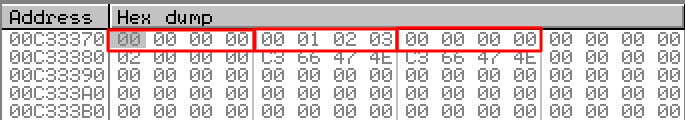
\includegraphics[scale=\NormalScale]{patterns/13_arrays/5_multidimensional/olly_2D_1.png}
\caption{\olly: \RU{массив заполнен}\EN{array is filled}}
\end{figure}

\subsubsection{\RU{Пример с заполнением столбца}\EN{Column filling example}}
\index{\olly}

\RU{Заполняем третий столбец значениями}\EN{Let's fill the third column with values:} $0 \ldots 2$.

\lstinputlisting[caption=\RU{Пример с заполнением столбца}\EN{Column filling example}]{patterns/13_arrays/5_multidimensional/two2.c.\LANG}

\RU{Здесь я также обвел красным три строки}\EN{I also marked three rows by red here}. 
\RU{Видно что в каждой строке, на третьей позиции, теперь записаны}
\EN{We see that in each row, at third position, these values are written:} 0, 1 \AndENRU 2.

\begin{figure}[H]
\centering
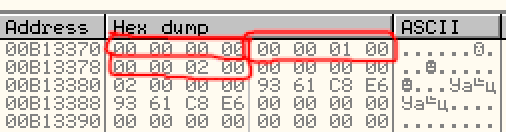
\includegraphics[scale=\NormalScale]{patterns/13_arrays/5_multidimensional/olly_2D_2.png}
\caption{\olly: \RU{массив заполнен}\EN{array is filled}}
\end{figure}

\subsection{\RU{Работа с двухмерным массивом как с одномерным}
\EN{Access two-dimensional array as one-dimensional}}

\RU{Мы можем легко убедиться, что можно работать с двухмерным массивом как с одномерным,
используя по крайней мере два метода:}
\EN{We can be easily assured that it's possible to access a two-dimensional array as one-dimensional array in at least two ways:}

\lstinputlisting{patterns/13_arrays/5_multidimensional/2D_as_1D.c.\LANG}

\RU{Компилируете и запускаете: мы увидим корректные значения.}
\EN{Compile and run it: it shows correct values.}

\RU{Очарователен результат работы MSVC 2013~--- все три процедуры одинаковые!}
\EN{What MSVC 2013 did is fascinating, all three routines are just the same!}

\lstinputlisting[caption=\Optimizing MSVC 2013 x64]{patterns/13_arrays/5_multidimensional/2D_as_1D_MSVC_2013_Ox_x64.asm.\LANG}

\RU{GCC сгенерировал практически одинаковые процедуры:}
\EN{GCC also generates equivalent routines, but slightly different:}

\lstinputlisting[caption=\Optimizing GCC 4.9 x64]{patterns/13_arrays/5_multidimensional/2D_as_1D_GCC49_x64_O3.s.\LANG}

\subsection{\RU{Пример с трехмерным массивом}\EN{Threedimensional array example}}

\RU{То же самое и для многомерных массивов.}\EN{Same thing about multidimensional arrays.}

\RU{На этот раз будем работать с массивом типа \Tint: каждый элемент требует 4 байта в памяти.}
\EN{Now we will work with array of \Tint type: each element require 4 bytes in memory.}

\RU{Попробуем}\EN{Let's see}:

\lstinputlisting[caption=\RU{простой пример}\EN{simple example}]{patterns/13_arrays/5_multidimensional/multi.c}

\subsubsection{x86}

\RU{В итоге}\EN{We got} (MSVC 2010):

\lstinputlisting[caption=MSVC 2010]{patterns/13_arrays/5_multidimensional/multi_msvc.asm}

\RU{В принципе, ничего удивительного. В \TT{insert()} для вычисления адреса нужного элемента массива, 
три входных аргумента перемножаются по формуле $address=600 \cdot 4 \cdot x + 30 \cdot 4 \cdot y + 4z$, 
чтобы представить массив трехмерным.
Не забывайте также, что тип \Tint 32-битный (4 байта), поэтому все коэффициенты нужно умножить на 4.}
\EN{Nothing special. For index calculation, three input arguments are multiplying 
by formula $address=600 \cdot 4 \cdot x + 30 \cdot 4 \cdot y + 4z$ to represent array as multidimensional.
Do not forget the \Tint type is 32-bit (4 bytes),
so all coefficients must be multiplied by 4.}

\lstinputlisting[caption=GCC 4.4.1]{patterns/13_arrays/5_multidimensional/multi_gcc.asm}

\RU{Компилятор GCC решил всё сделать немного иначе}\EN{GCC compiler does it differently}.
\RU{Для вычисления одной из операций ($30y$), GCC создал код, где нет самой операции умножения.}
\EN{For one of operations calculating ($30y$), GCC produced a code without multiplication instruction.}
\RU{Происходит это так}\EN{This is how it done}: 
$(y+y) \ll 4 - (y+y) = (2y) \ll 4 - 2y = 2 \cdot 16 \cdot y - 2y = 32y - 2y = 30y$. 
\RU{Таким образом, для вычисления $30y$ используется только операция сложения, 
операция битового сдвига и операция вычитания.}\EN{Thus, for $30y$ calculation, only one addition operation
used, one bitwise shift operation and one subtraction operation.}
\RU{Это работает быстрее}\EN{That works faster}.

\subsubsection{ARM + \NonOptimizingXcodeIV (\ThumbMode)}

\lstinputlisting[caption=\NonOptimizingXcodeIV (\ThumbMode)]{patterns/13_arrays/5_multidimensional/multi_Xcode_thumb_O0_\LANG.asm}

\NonOptimizing LLVM \RU{сохраняет все переменные в локальном стеке, хотя это и избыточно.}
\EN{saves all variables in local stack, however, it is redundant.}
\RU{Адрес элемента массива вычисляется по уже рассмотренной формуле.}
\EN{Address of array element is calculated by formula we already figured out.}

\subsubsection{ARM + \OptimizingXcodeIV (\ThumbMode)}

\lstinputlisting[caption=\OptimizingXcodeIV (\ThumbMode)]{patterns/13_arrays/5_multidimensional/multi_Xcode_thumb_O3_\LANG.asm}

\RU{Тут используются уже описанные трюки для замены умножения на операции сдвига, сложения и вычитания.}
\EN{Here is used tricks for replacing multiplication by shift, addition and subtraction we already considered.}

\index{ARM!\Instructions!RSB}
\index{ARM!\Instructions!SUB}
\RU{Также мы видим новую для себя инструкцию}\EN{Here we also see new instruction for us:} 
\TT{RSB} (\IT{Reverse Subtract}).
\RU{Она работает так же, как и \SUB, только меняет операнды местами.}
\EN{It works just as \SUB, but swapping operands with each other.}
\RU{Зачем?}\EN{Why?}
\index{ARM!Optional operators!LSL}
\SUB, \TT{RSB}, \RU{это те инструкции, ко второму операнду которых можно применить коэффициент сдвига, 
как мы видим и здесь}
\EN{are those instructions, to the second operand of which shift coefficient may be applied}: (\TT{LSL\#4}). 
\RU{Но этот коэффициент можно применить только ко второму операнду.}
\EN{But this coefficient may be applied only to second operand.}
\RU{Для коммутативных операций, таких как сложение или умножение, 
там операнды можно менять местами и это не влияет на результат.}
\EN{That's fine for commutative operations like addition or multiplication, operands may be swapped there
without result affecting.}
\RU{Но вычитание ~--- операция некоммутативная, так что, для этих случаев существует инструкция \TT{RSB}.}
\EN{But subtraction is non-commutative operation, so, for these cases, \TT{RSB} exist.}

\index{ARM!\Instructions!LDR.W}
\RU{Инструкция }\TT{``LDR.W R9, [R9]''} \RU{работает как}\EN{instruction works like} \LEA~(\ref{sec:LEA})
\RU{в x86, и здесь она ничего не делает, она избыточна.}\EN{in x86, but here it does nothing, it is redundant.}
\RU{Вероятно, компилятор несоптимизировал её.}\EN{Apparently, compiler not optimized it.}



\ifx\LITE\undefined
\subsection{\RU{Еще примеры}\EN{More examples}}

\RU{Компьютерный экран представляет собой двухмерный массив, но видеобуфер это линейный
одномерный массив}\EN{The computer screen is represented as a 2D array, but the video-buffer is 
a linear 1D array}. 
\RU{Мы рассматриваем это здесь}\EN{We talk about it here}: \myref{Mandelbrot_demo}.
\fi

\ifx\LITE\undefined
\section{\RU{Набор строк как двухмерный массив}\EN{Pack of strings as a two-dimensional array}}

\RU{Снова вернемся к примеру, который возвращает название месяца:}
\EN{Let's revisit the function that returns the name of a month:} \lstref{get_month1}.
\RU{Как видно, нужна как минимум одна операция загрузки из памяти для подготовки указателя на строку,
состоящую из имени месяца.}
\EN{As you see, at least one memory load operation is needed to prepare a pointer to the string
that's the month's name.}
\RU{Возможно ли избавиться от операции загрузки из памяти?}
\EN{Is it possible to get rid of this memory load operation?}
\RU{На самом деле, да, если представить список строк как двухмерный массив:}
\EN{In fact yes, if you represent the list of strings as a two-dimensional array:}

\lstinputlisting{patterns/13_arrays/55_month_2D/month2.c.\LANG}

\RU{Вот что получаем:}\EN{Here is what we've get:}

\lstinputlisting[caption=\Optimizing MSVC 2013 x64]{patterns/13_arrays/55_month_2D/MSVC2013_x64_Ox.asm.\LANG}

\RU{Здесь нет обращений к памяти вообще}\EN{There are no memory accesses at all}.
\RU{Всё что делает эта функция это вычисляет место, где находится первый символ названия месяца:}
\EN{All this function does is to calculate a point at which the first character of the name of the month is:} 
$pointer\_to\_the\_table + month * 10$.
\RU{Там также две инструкции LEA, которые работают как несколько инструкций MUL и MOV.}
\EN{There are also two LEA instructions, which effectively work as several MUL and MOV instructions.}

\RU{Ширина массива --- 10 байт}\EN{The width of the array is 10 bytes}. 
\RU{Действительно, самая длинная строка здесь это \q{September} (9 байт) плюс оконечивающий ноль --- это 10 байт.}
\EN{Indeed, the longest string here --- \q{September} --- is 9 bytes, and plus the terminating zero is 10 bytes.}
\RU{Остальные названия месяцев дополнены нулевыми байтами, чтобы они занимали столько же места (10 байт).}
\EN{The rest of the month names are padded by zero bytes, so they all occupy the same space (10 bytes).}
\RU{Таким образом, наша функция и работает быстрее, потому что все строки начинаются с тех адресов, 
которые легко вычислить.}
\EN{Thus, our function works even faster, because all string start at an address which can be
calculated easily.}

\Optimizing GCC 4.9 \RU{может еще короче}\EN{can do it even shorter}:

\begin{lstlisting}[caption=\Optimizing GCC 4.9 x64]
	movsx	rdi, edi
	lea	rax, [rdi+rdi*4]
	lea	rax, month2[rax+rax]
	ret
\end{lstlisting}

\RU{LEA здесь также используется для умножения на 10.}
\EN{LEA is also used here for multiplication by 10.}

\RU{Неоптимизирующие компиляторы делают умножение по-разному.}
\EN{Non-optimizing compilers do multiplication differently.}

\lstinputlisting[caption=\NonOptimizing GCC 4.9 x64]{patterns/13_arrays/55_month_2D/x64_GCC49_O0.asm.\LANG}

\NonOptimizing MSVC \RU{просто использует инструкцию IMUL}\EN{just use IMUL instruction}:
\index{x86!\Instructions!IMUL}

\lstinputlisting[caption=\NonOptimizing MSVC 2013 x64]{patterns/13_arrays/55_month_2D/MSVC2013_x64.asm.\LANG}

\index{\CompilerAnomaly}
\label{MSVC2013_anomaly}
\dots \RU{но вот что странно: зачем добавлять умножение на ноль и добавлять ноль к конечному результату?}
\EN{but one thing is weird here: why add multiplication by zero and adding zero to the final result?}
\RU{Я не знаю, это выглядит как выверт кодегенератора компилятора, который не был покрыт тестами
компилятора (так или иначе, итоговый код работает корректно).}
\EN{I don't know, this looks like a compiler code generator quirk, which wasn't caught by the compiler's tests
(the resulting code works correctly, after all).}
\RU{Я сознательно добавляю сюда такие фрагменты кода, чтобы читатель понимал, что иногда не нужно
ломать себе голову над подобными артефактами компиляторов.}
\EN{I intentionally add such pieces of code so the reader would understand, 
that sometimes one shouldn't puzzle over such compiler artifacts.}

\ifdefined\IncludeARM
\subsection{32-bit ARM}

\Optimizing Keil \RU{для режима Thumb использует инструкцию умножения}
\EN{for Thumb mode uses the multiplication instruction} MULS:

\lstinputlisting[caption=\OptimizingKeilVI (\ThumbMode)]{patterns/13_arrays/55_month_2D/Keil_O3_thumb.asm.\LANG}

\Optimizing Keil \RU{для режима ARM использует операции сложения и сдвига}\EN{for ARM mode uses add and 
shift operations}:

\lstinputlisting[caption=\OptimizingKeilVI (\ARMMode)]{patterns/13_arrays/55_month_2D/Keil_O3_ARM.asm.\LANG}

\subsection{ARM64}

\lstinputlisting[caption=\Optimizing GCC 4.9 ARM64]{patterns/13_arrays/55_month_2D/GCC49_ARM64.asm.\LANG}

\index{ARM!\Instructions!SXTW}
\index{ARM!\Instructions!ADRP/ADD pair}
\RU{SXTW используется для знакового расширения и расширения входного 32-битного значения в 64-битное и сохранения
его в X0.}
\EN{SXTW is used for sign-extension and promoting input 32-bit value into a 64-bit one and storing it in X0.}
\RU{Пара ADRP/ADD используется для загрузки адреса таблицы.}
\EN{ADRP/ADD pair is used for loading the address of the table.}
\RU{У инструкции ADD также есть суффикс LSL, что помогает с умножением.}
\EN{The ADD instructions also has a LSL suffix, which helps with multiplications.}
\fi

\ifdefined\IncludeMIPS
\subsection{MIPS}
\lstinputlisting[caption=\Optimizing GCC 4.4.5 (IDA)]{patterns/13_arrays/55_month_2D/MIPS_O3_IDA.lst.\LANG}
\fi

\subsection{\Conclusion{}}

\RU{Это немного олд-скульная техника для хранения текстовых строк.}
\EN{This is a bit old-school technique to store text strings.}
\RU{Такого можно много найти в \oracle, например.}
\EN{You may find a lot of it in \oracle, for example.}
\RU{Но я не уверен, стоит ли оно того на современных компьютерах.}
\EN{But I don't really know if it's worth doing on modern computers.}
\RU{Так или иначе, это был хороший пример массивов, так что я добавил его в эту книгу.}
\EN{Nevertheless, it was a good example of arrays, so I added it to this book.}

\fi
\subsection{\Conclusion{}}

\RU{Массив это просто набор значений в памяти, расположенных рядом друг с другом.}
\EN{An array is a pack of values in memory located adjacently.}
\RU{Это справедливо для любых типов элементов, включая структуры.}
\EN{It's true for any element type, including structures.}
\RU{Доступ к определенному элементу массива это просто вычисление его адреса.}
\EN{Access to a specific array element is just a calculation of its address.}

\ifdefined\IncludeExercises
\section{\Exercises}

\subsection{\Exercise \#1}
% matrix addition
\label{exercise_array_1}

\WhatThisCodeDoes\

\lstinputlisting[caption=MSVC 2010 + \TT{/O1}]{patterns/13_arrays/exercises/1_msvc.asm}

(/O1: \RU{оптимизация по размеру кода}\EN{minimize space}).

\lstinputlisting[caption=Keil 5.03 (\ARMMode) + \Othree]{patterns/13_arrays/exercises/1_ARM.s}

\lstinputlisting[caption=Keil 5.03 (\ThumbMode) + \Othree]{patterns/13_arrays/exercises/1_thumb.s}

\Answer\: \ref{exercise_solutions_arrays_1}.

\subsection{\Exercise \#2}
% matrix multiplication
\label{exercise_array_2}

\WhatThisCodeDoes\

\lstinputlisting[caption=MSVC 2010 + \TT{/O1}]{patterns/13_arrays/exercises/2_msvc.asm}

(/O1: \RU{оптимизация по размеру кода}\EN{minimize space}).

\lstinputlisting[caption=Keil 5.03 (\ARMMode) + \Othree]{patterns/13_arrays/exercises/2_ARM.s}

\lstinputlisting[caption=Keil 5.03 (\ThumbMode) + \Othree]{patterns/13_arrays/exercises/2_thumb.s}

\Answer\: \ref{exercise_solutions_arrays_2}.

\subsection{\Exercise \#3}
\label{exercise_array_3}

\WhatThisCodeDoes\

\EN{Try to determine array size, at least partially.}
\RU{Попробуйте определить размеры массива, хотя бы частично.}

\begin{lstlisting}[caption=MSVC 2010 /Ox]
_array$ = 8
_x$ = 12
_y$ = 16
_f	PROC
	mov	eax, DWORD PTR _x$[esp-4]
	mov	edx, DWORD PTR _y$[esp-4]
	mov	ecx, eax
	shl	ecx, 4
	sub	ecx, eax
	lea	eax, DWORD PTR [edx+ecx*8]
	mov	ecx, DWORD PTR _array$[esp-4]
	fld	QWORD PTR [ecx+eax*8]
	ret	0
_f	ENDP
\end{lstlisting}

\begin{lstlisting}[caption=Keil 5.03 (\ARMMode)]
f PROC
        RSB      r1,r1,r1,LSL #4
        ADD      r0,r0,r1,LSL #6
        ADD      r1,r0,r2,LSL #3
        LDM      r1,{r0,r1}
        BX       lr
        ENDP
\end{lstlisting}

\begin{lstlisting}[caption=Keil 5.03 (\ThumbMode)]
f PROC
        MOVS     r3,#0xf
        LSLS     r3,r3,#6
        MULS     r1,r3,r1
        ADDS     r0,r1,r0
        LSLS     r1,r2,#3
        ADDS     r1,r0,r1
        LDM      r1,{r0,r1}
        BX       lr
        ENDP
\end{lstlisting}

\Answer\: \ref{exercise_solutions_arrays_3}

\subsection{\Exercise \#4}
\label{exercise_array_4}

\WhatThisCodeDoes\

\EN{Try to determine array size, at least partially.}
\RU{Попробуйте определить размеры массива, хотя бы частично.}

\begin{lstlisting}[caption=MSVC 2010 /Ox]
_array$ = 8	
_x$ = 12	
_y$ = 16	
_z$ = 20	
_f	PROC
	mov	eax, DWORD PTR _x$[esp-4]
	mov	edx, DWORD PTR _y$[esp-4]
	mov	ecx, eax
	shl	ecx, 4
	sub	ecx, eax
	lea	eax, DWORD PTR [edx+ecx*4]
	mov	ecx, DWORD PTR _array$[esp-4]
	lea	eax, DWORD PTR [eax+eax*4]
	shl	eax, 4
	add	eax, DWORD PTR _z$[esp-4]
	mov	eax, DWORD PTR [ecx+eax*4]
	ret	0
_f	ENDP
\end{lstlisting}

\begin{lstlisting}[caption=Keil 5.03 (\ARMMode)]
f PROC
        RSB      r1,r1,r1,LSL #4
        ADD      r1,r1,r1,LSL #2
        ADD      r0,r0,r1,LSL #8
        ADD      r1,r2,r2,LSL #2
        ADD      r0,r0,r1,LSL #6
        LDR      r0,[r0,r3,LSL #2]
        BX       lr
        ENDP
\end{lstlisting}

\begin{lstlisting}[caption=Keil 5.03 (\ThumbMode)]
f PROC
        PUSH     {r4,lr}
        MOVS     r4,#0x4b
        LSLS     r4,r4,#8
        MULS     r1,r4,r1
        ADDS     r0,r1,r0
        MOVS     r1,#0xff
        ADDS     r1,r1,#0x41
        MULS     r2,r1,r2
        ADDS     r0,r0,r2
        LSLS     r1,r3,#2
        LDR      r0,[r0,r1]
        POP      {r4,pc}
        ENDP
\end{lstlisting}

\Answer\: \ref{exercise_solutions_arrays_4}

\subsection{\Exercise \#5}
\label{exercise_array_5}

\WhatThisCodeDoes\

\begin{lstlisting}[caption=MSVC 2012 /Ox /GS-]
COMM	_tbl:DWORD:064H

tv759 = -4	; size = 4
_main	PROC
	push	ecx
	push	ebx
	push	ebp
	push	esi
	xor	edx, edx
	push	edi
	xor	esi, esi
	xor	edi, edi
	xor	ebx, ebx
	xor	ebp, ebp
	mov	DWORD PTR tv759[esp+20], edx
	mov	eax, OFFSET _tbl+4
	npad	8
$LL6@main:
	lea	ecx, DWORD PTR [edx+edx]
	mov	DWORD PTR [eax+4], ecx
	mov	ecx, DWORD PTR tv759[esp+20]
	add	DWORD PTR tv759[esp+20], 3
	mov	DWORD PTR [eax+8], ecx
	lea	ecx, DWORD PTR [edx*4]
	mov	DWORD PTR [eax+12], ecx
	lea	ecx, DWORD PTR [edx*8]
	mov	DWORD PTR [eax], edx
	mov	DWORD PTR [eax+16], ebp
	mov	DWORD PTR [eax+20], ebx
	mov	DWORD PTR [eax+24], edi
	mov	DWORD PTR [eax+32], esi
	mov	DWORD PTR [eax-4], 0
	mov	DWORD PTR [eax+28], ecx
	add	eax, 40
	inc	edx
	add	ebp, 5
	add	ebx, 6
	add	edi, 7
	add	esi, 9
	cmp	eax, OFFSET _tbl+404
	jl	SHORT $LL6@main
	pop	edi
	pop	esi
	pop	ebp
	xor	eax, eax
	pop	ebx
	pop	ecx
	ret	0
_main	ENDP
\end{lstlisting}

\begin{lstlisting}[caption=Keil 5.03 (\ARMMode)]
main PROC
        LDR      r12,|L0.60|
        MOV      r1,#0
|L0.8|
        ADD      r2,r1,r1,LSL #2
        MOV      r0,#0
        ADD      r2,r12,r2,LSL #3
|L0.20|
        MUL      r3,r1,r0
        STR      r3,[r2,r0,LSL #2]
        ADD      r0,r0,#1
        CMP      r0,#0xa
        BLT      |L0.20|
        ADD      r1,r1,#1
        CMP      r1,#0xa
        MOVGE    r0,#0
        BLT      |L0.8|
        BX       lr
        ENDP

|L0.60|
        DCD      ||.bss||

        AREA ||.bss||, DATA, NOINIT, ALIGN=2

tbl
        %        400
\end{lstlisting}

\begin{lstlisting}[caption=Keil 5.03 (\ThumbMode)]
main PROC
        PUSH     {r4,r5,lr}
        LDR      r4,|L0.40|
        MOVS     r1,#0
|L0.6|
        MOVS     r2,#0x28
        MULS     r2,r1,r2
        MOVS     r0,#0
        ADDS     r3,r2,r4
|L0.14|
        MOVS     r2,r1
        MULS     r2,r0,r2
        LSLS     r5,r0,#2
        ADDS     r0,r0,#1
        CMP      r0,#0xa
        STR      r2,[r3,r5]
        BLT      |L0.14|
        ADDS     r1,r1,#1
        CMP      r1,#0xa
        BLT      |L0.6|
        MOVS     r0,#0
        POP      {r4,r5,pc}
        ENDP

        DCW      0x0000
|L0.40|
        DCD      ||.bss||

        AREA ||.bss||, DATA, NOINIT, ALIGN=2

tbl
        %        400
\end{lstlisting}

\Answer\: \ref{exercise_solutions_arrays_5}

\fi
